% Latex template: mahmoud.s.fahmy@students.kasralainy.edu.eg
% For more details: https://www.sharelatex.com/learn/Beamer

\documentclass[aspectratio=1610]{beamer}					% Document class

\setbeamertemplate{footline}[text line]{%
  \parbox{\linewidth}{\vspace*{-8pt}Predictive spatial models of gene regulation via Bayesian inference \hfill\insertshortauthor\hfill\insertpagenumber}}
\setbeamertemplate{navigation symbols}{}

\usepackage[english]{babel}				% Set language
\usepackage[utf8x]{inputenc}			% Set encoding

\mode<presentation>						% Set options
{
  \usetheme{default}					% Set theme
  \usecolortheme{default} 				% Set colors
  \usefonttheme{default}  				% Set font theme
  \setbeamertemplate{caption}[numbered]	% Set caption to be numbered
}

% Uncomment this to have the outline at the beginning of each section highlighted.
%\AtBeginSection[]
%{
%  \begin{frame}{Outline}
%    \tableofcontents[currentsection]
%  \end{frame}
%}

\usepackage{graphicx}					% For including figures
\usepackage{booktabs}					% For table rules
\usepackage{hyperref}	
\usepackage{tikz-network}				% For cross-referencing
\usepackage[absolute,overlay]{textpos}
\usepackage{bm}
\usepackage[font=small,labelfont=bf]{caption}

\title{Predictive spatial models of gene regulation via Bayesian inference}	% Presentation title
\author{Clayton W. Seitz}								% Presentation author
\date{\today}									% Today's date	

\begin{document}

% Title page
% This page includes the informations defined earlier including title, author/s, affiliation/s and the date
\begin{frame}
  \titlepage
\end{frame}


% The following is the most frequently used slide types in beamer
% The slide structure is as follows:
%
%\begin{frame}{<slide-title>}
%	<content>
%\end{frame}

\begin{frame}{Gene expression is stochastic and non-constitutive}


\begin{textblock*}{7cm}(0.5cm,1cm)
\begin{figure}
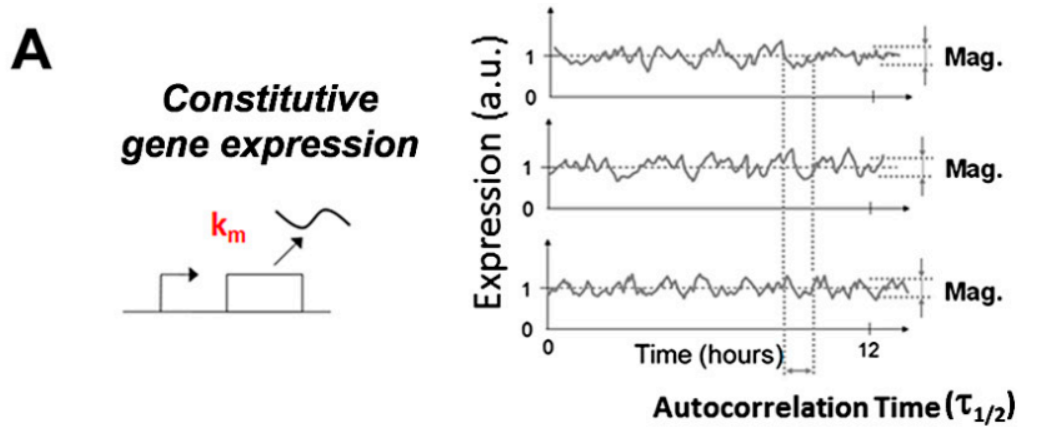
\includegraphics[width=7cm]{burst-1.png}
\end{figure}
\end{textblock*}

\begin{textblock*}{7cm}(8cm,1cm)
\begin{figure}
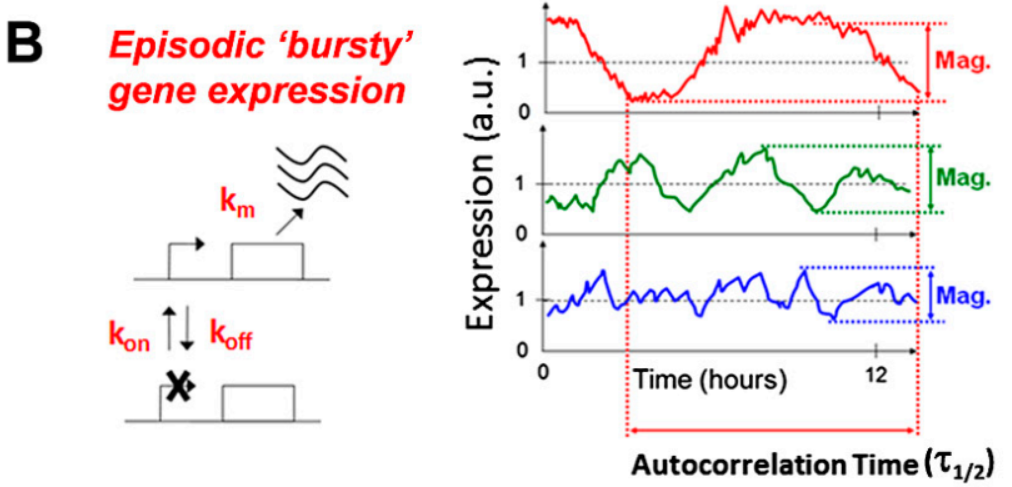
\includegraphics[width=7cm]{burst-2.png}
\end{figure}
\end{textblock*}


\begin{textblock*}{15cm}(0.5cm,5cm)
\textbf{Single-state models}
\begin{itemize}
\item Transcription occurs at a fixed rate
\item mRNA counts are Poisson
\item \textcolor{red}{Underestimates variance in mRNA counts}
\end{itemize}
\end{textblock*}
\begin{textblock*}{15cm}(8.5cm,5cm)
\textbf{Two-state models}
\begin{itemize}
\item Promoter can be on or off
\item mRNA counts are not Poisson
\end{itemize}

\end{textblock*}

\begin{textblock*}{15cm}(0.5cm,8cm)
Chromatin structure is complicated e.g., loops. Multiple \emph{cis}-regulatory elements can contribute to promoter switching and transcription control
\end{textblock*}

\end{frame}

\begin{frame}{STL1/CTT1 induction with NaCl in yeast}
\begin{textblock*}{12cm}(2cm,1.25cm)
\begin{figure}
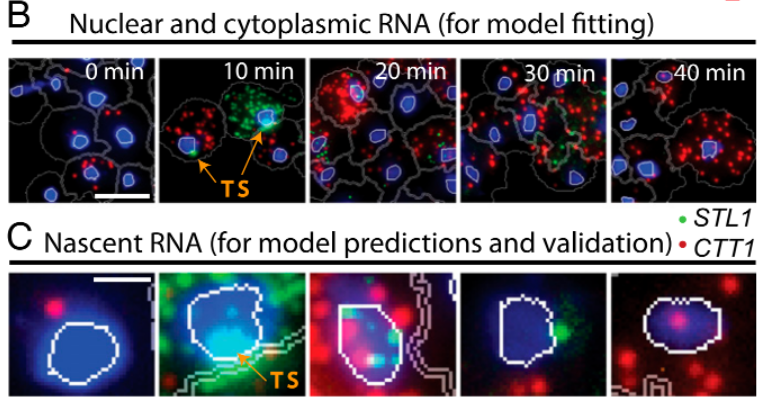
\includegraphics[width=12cm]{salt.png}
\caption{Munsky et al., PNAS 2018}
\end{figure}
\end{textblock*}
\end{frame}

\begin{frame}{A quick note on ergodicity and ensemble snapshots}
\begin{itemize}
\item \textcolor{red}{Ergodicity} = statistics of the ensemble and a single process are the same
\item Implies the parameters of the process are the same for every cell
\item Ensemble snapshots useful due to experimental constraints (multiplexing)
\end{itemize}
\begin{textblock*}{15cm}(0.5cm,7.25cm)

\begin{equation*}
\underset{N\rightarrow \infty}{\mathrm{lim}} \frac{1}{N}\sum_{i=1}^{N} (x_{i}-\mu)^{n} = \int (x-\mu)^{n} p(x)dx
\end{equation*}
\end{textblock*}

\end{frame}

\begin{frame}{A compartment model for spatial gene expression}
\begin{textblock*}{10cm}(3cm,1.25cm)
\begin{figure}
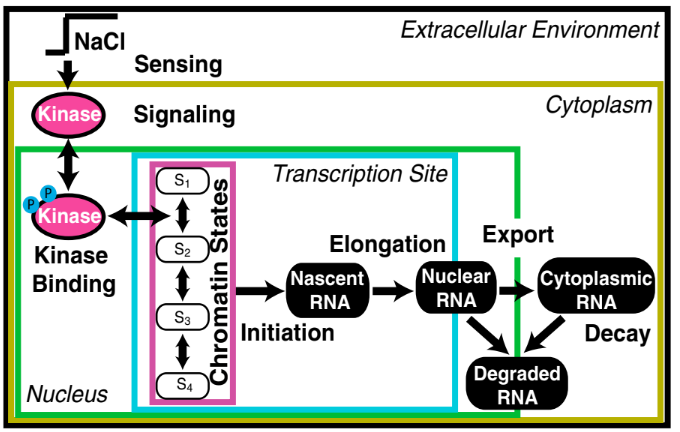
\includegraphics[width=10cm]{compartment.png}
\caption{Munsky et al., PNAS 2018}
\end{figure}
\end{textblock*}
\end{frame}

\begin{frame}{A compartment model for spatial gene expression}

Let $X$ represent an arbitrary RNA transcript of gene $G$

\begin{align*}
\mathrm{Gene\;activation}: G_{off} &\overset{k_{on}}{\rightarrow} G_{on}\\
\mathrm{Gene\;inactivation}: G_{off} &\overset{k_{off}}{\rightarrow} G_{on}\\
\mathrm{Transcription}: G_{on} &\overset{k_{t}}{\rightarrow} G_{on} + X_{\mathrm{nuc}}\\
\mathrm{RNA \;Export}: X_{\mathrm{nuc}} &\overset{k_{exp}}{\rightarrow} X_{\mathrm{cyt}}\\
\mathrm{RNA\; degradation}: X_{\mathrm{cyt}} &\overset{\gamma}{\rightarrow} \emptyset\\
\end{align*}

Raw data collected post induction can be used to infer parameters

\begin{equation*}
\theta = \left( k_{on},k_{off},k_{t},k_{exp},\gamma\right)
\end{equation*}

\end{frame}

\begin{frame}{Brownian RNA transport in the nucleus}

\begin{textblock*}{12cm}(2cm,1.25cm)
\begin{figure}
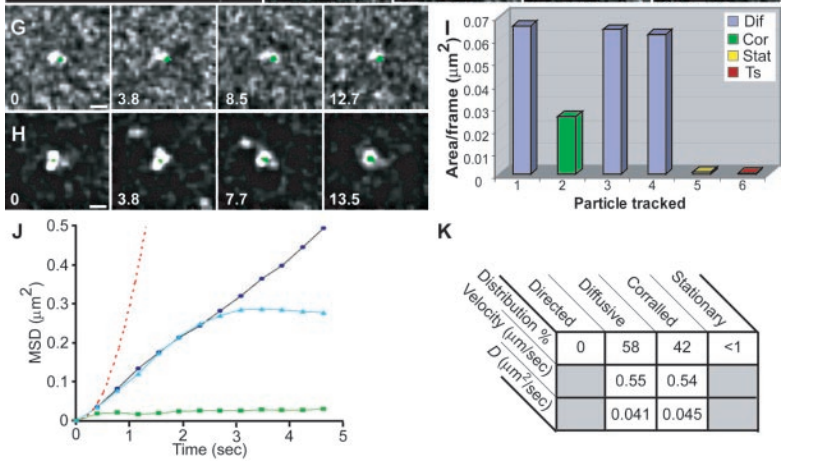
\includegraphics[width=12cm]{diffusion.png}
\caption{Shav-Tal et al., Science 2004}
\end{figure}
\end{textblock*}


\end{frame}

\begin{frame}{Rate of nuclear export is determined by diffusion}

The first passage time density (FPTD) determines the rate of RNA export\\
\vspace{0.1in}
Particles are distinguishable (non-ergodic dynamics) \\
\vspace{0.1in}
Brownian motion and ``corralled" motion raise questions about a constant export rate parameter

\end{frame}

\begin{frame}{An Ising model of promoter switching}

Promoter activation often requires chromatin reorganization, binding of specific TF combinations. We can imagine a random (?) walk through the binding phase space

\begin{align*}
\mathcal{H} = -\frac{1}{2}\sum_{i,j}J_{ij}x_{i}x_{j} - \sum_{j}h_{j}x_{j}\;\;\;\; P(\bm{x}) = \frac{1}{Z}\exp\left(-\beta \mathcal{H}(\bm{x})\right)
\end{align*}

We know $p(x_{j}=1) = \exp(-\beta H(x_{i}=1))$. Then, we define 

\begin{align*}
h_{j} = -\frac{1}{\beta}\log p(x_{i}=1) = -\frac{1}{\beta}\log \frac{[x_{j}]}{K_{j} + [x_{j}]}
\end{align*}

Suppose that there is a single state or set of states $\bm{x}^{*}$ for which the promoter is active

\begin{align*}
\lambda = \frac{Z_{on}}{Z_{on}+Z_{off}} \;\;\rightarrow\;\; P(n|\mu) = \frac{\mu^{n}}{n!}\exp(-\mu)
\end{align*}

with $\mu=\lambda t$

\end{frame}

\begin{frame}{Bayesian parameter inference using ensemble snapshots}

Suppose we have a series of ensemble snapshots of an \emph{in-vitro} population:

\begin{align*}
\mathbf{x} = \{\mathbf{x}_{0}, ..., \mathbf{x}_{t}\}\;\;\; \mathbf{y} = \{\mathbf{y}_{0}, ..., \mathbf{y}_{t}\}
\end{align*}

with $\mathbf{x}_{t} = \{x_{1}, ..., x_{n}\}$ and similarly for $\mathbf{y}$. Under perfect measurements $\mathbf{x}=\mathbf{y}$\\
\vspace{0.2in}
We would like to use $\mathbf{x}$ to fit a dynamical model $\mathcal{M}(\theta)$. Bayesian inference lets us infer $\theta$ from $\mathbf{x}$ while quantifying the uncertainty in our estimate:

\begin{align*}
P(\theta|\mathbf{x}) \propto f(\mathbf{x}|\theta)\pi(\theta) = \pi(\theta)\prod_{t} f(\mathbf{x}_{t}|\theta)
\end{align*}

The likelihood $f(\mathbf{x}_{t}|\theta)$ is often difficult to define or intractable to compute due to the curse of dimensionality, making even MLE a challenge

\end{frame}


\begin{frame}{Kolmogorov's forward equation (chemical master equation)}

Dynamics on biochemical reaction networks are inherently stochastic and the state space is discrete. We can only write probabilities over the state space

\vspace{0.1in}

\begin{align*}
P(\mathbf{x}_{i},t) &= \sum_{j} T_{ji}(\mathbf{x}_{i},t|\mathbf{x}_{j},t-\Delta t)P(\mathbf{x}_{j},t-\Delta t)\\ 
&= \sum_{k} T_{k}(\mathbf{x}_{i},t|\mathbf{x}_{i}-\nu_{k},t-\Delta t)P(\mathbf{x}_{i}-\nu_{k},t-\Delta t)
\end{align*}

where $T_{k}$ is the probability of a reaction channel $k$ firing in the interval $(t,t+\Delta t)$.\\
\vspace{0.1in}
Taking the limit $\Delta t \rightarrow 0$ one can derive the forward Kolmogorov equation or chemical master equation (CME)

\begin{align*}
\frac{dP(\mathbf{x},t|\mathbf{x}_{0})}{dt} = \sum_{k} T_{k}(\mathbf{x}-\nu_{k})P(\mathbf{x}-\nu_{k},t) - T_{k}(\mathbf{x})P(\mathbf{x},t)
\end{align*}

\end{frame}


% Adding the option 'allowframebreaks' allows the contents of the slide to be expanded in more than one slide.
\begin{frame}[allowframebreaks]{References}
	\tiny\bibliography{references}
	\bibliographystyle{apalike}
\end{frame}

\end{document}
